\documentclass[../Article_Model_Parameters.tex]{subfiles}
\graphicspath{{\subfix{../Figures/}}}
\begin{document}
	
	%\footnote{For the sake of clarity of the process model, different colors have been used in the equations to indicate: 
		%	{\color{red}control variables},
		%	{\color{black}state variables},
		%	{\color{black}variables} and
		%	{\color{black}parameters}.} 
	The governing equation for a quasi-one-dimensional compressible flow in Cartesian coordinates can be found in the Appendix \ref{CH: Gouverning equations} and in the work of \citet{Anderson1995}. Quasi-one-dimensional flow is a fluid flow characterized by the assumption that the flow properties remain uniform across any given cross-section of the flow. This assumption is made when there is a variation in the cross-sectional area of the flow channel, such as an irregular shape or partial filling of an extractor. In such cases, the flow is considered to be quasi-one-dimensional because the velocity and other flow properties are assumed to vary only in the direction of flow.
	
	The quasi-one-dimensional compressible Navier-Stokes equations in Cartesian coordinates are given by Equations \ref{EQ: CompressibleEuler_1} to \ref{EQ: CompressibleEuler_3}. The derivation of these Equations are presented in Appendix \ref{CH: Gouverning equations}.
	
	{\footnotesize
		\begin{align}
			\label{EQ: CompressibleEuler_1}
			\cfrac{\partial \left( {\color{black}\rho_f} {\color{black}A_f}(z) \right) }{\partial t} + \cfrac{\partial \left( {\color{black}\rho_f} {\color{black}A_f}(z) v \right)}{\partial z} &= 0 \\
			\cfrac{\partial \left( {\color{black}\rho_f} v {\color{black}A_f}(z) \right) }{\partial t} + \cfrac{\partial \left( {\color{black}\rho_f} {\color{black}A_f}(z) v^2 \right)}{\partial z} &= -{\color{black}A_f}(z) \cfrac{\partial {\color{black}P}}{\partial z} \label{EQ: CompressibleEuler_2} \\
			\cfrac{\partial \left( {\color{black}\rho_f} {\color{black}e} {\color{black}A_f}(z) \right) }{\partial t} + \cfrac{\partial \left( {\color{black}\rho_f} {\color{black}A_f}(z) v {\color{black}e}\right)}{\partial z} &= -{\color{black}P}\cfrac{\left( {\color{black}A_f}(z) v \right)}{\partial z} + \cfrac{\partial}{\partial z} \left( \cfrac{\partial {\color{black}T}}{\partial z} \right)   
			\label{EQ: CompressibleEuler_3}
		\end{align}  
	}
	
	where ${\color{black}\rho_f}$ is the density of the fluid, ${\color{black}A_f}(z)$ is the function which describe change of the cross-section, $v$ is the velocity, ${\color{black}P}$ is the total pressure, ${\color{black}e}$ is the internal energy of the fluid, $t$ is time and $z$ is the spacial direction.
	
	Based on governing equations, the small discontinuity (defined as $\delta$) in flow properties, shown in Figure \ref{fig: Discontinuity_slow_flow}, can be analysed. The analysis follows the work of \citet{Schreier1982}.
	
	\begin{figure}[!h]
		\centering
		\resizebox{0.95\columnwidth}{!}{%
			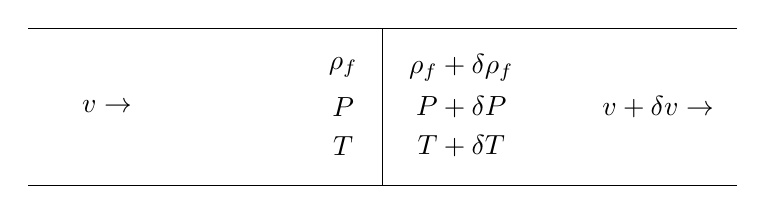
\begin{tikzpicture}[]
				\draw (0,2) -- (9,2);	% Top line
				\draw (0,0) -- (9,0); 	% Bottom line
				\draw (4.5,0) -- (4.5,2); 	% Bottom line
				\node at (4,1.5) {${\color{black}\rho_f}$};
				\node at (5.5,1.5) {${\color{black}\rho_f}+\delta{\color{black}\rho_f}$};
				\node at (4,1.0) {${\color{black}P}$};
				\node at (5.5,1.0) {${\color{black}P}+\delta {\color{black}P}$};
				\node at (4,0.5) {${\color{black}T}$};
				\node at (5.5,0.5) {${\color{black}T}+\delta {\color{black}T}$};
				\node at (1,1.0) {$v \rightarrow$};
				\node at (8,1.0) {$v + \delta v \rightarrow$};
		\end{tikzpicture} }
		\caption{Small discontinuity in one-dimensional flow}
		\label{fig: Discontinuity_slow_flow}
	\end{figure} 
	
	The discontinuity is presumed to be at rest relative, and the balance equations become		
	
	{\footnotesize
		\begin{align*}
			&{\color{black}\rho_f} \delta v + v \delta {\color{black}\rho_f} + \delta {\color{black}\rho_f} \delta v = 0 \\
			&\delta {\color{black}P} = \delta v \delta {\color{black}\rho_f}
		\end{align*}
	}
	
	These relations are equally valid if the two regions are separated by a region of finite width rather than a discontinuity. 
	
	{\footnotesize
		\begin{equation*}
			\lim_{{\color{black}\rho_f} v \rightarrow 0} {\color{black}\rho_f} \delta v + v \delta {\color{black}\rho_f} + \delta {\color{black}\rho_f} \delta v = 0 / \delta {\color{black}\rho_f} \rightarrow \cfrac{d v}{d {\color{black}\rho_f}} = - \cfrac{v}{{\color{black}\rho_f}}
		\end{equation*}
	}
	
	By combining the momentum equation with the above equation, we get
	
	{\footnotesize
		\begin{equation} \label{EQ: Pressure_Velocity}
			\cfrac{d v}{d {\color{black}\rho_f}} = - \cfrac{d v}{d{\color{black}P}} \cfrac{d {\color{black}P}}{d {\color{black}\rho_f}} = -\cfrac{1}{\rho v} \cfrac{d{\color{black}P}}{d{\color{black}\rho_f}} = -\cfrac{v}{{\color{black}\rho_f}}
		\end{equation}
	}
	
	Suppose the flow is presumed to be isentropic, $d{\color{black}P}/d{\color{black}\rho_f} = c^2$, so $v^2=c^2$, where $c$ is the speed of sound. This can be interpreted as a small pressure wave propagating with the speed of sound relative to the flow. Moreover, if the flow velocity is relatively low, all pressure changes are hydrodynamic (due to velocity motion) rather than thermodynamic which leads to $\partial {\color{black}\rho_f} / \partial {\color{black}P} \approx 0$. In other words, the small changes in pressure due to flow velocity changes do not change the density. %This has a secondary effect -- the speed of sound in the fluid is $\partial {\color{black}P}/\partial {\color{black}\rho_f} = \infty$ in this instance. So there is an infinite speed of sound, which makes the equations elliptic in nature. It can be deduced that at the isothermal conditions, the density in the system propagates with the same speed as pressure since they are both connected through the equation of state. The details of the Mach-number analysis are presented in Appendix \ref{CH:Low_Mach_chapter}.

\end{document}